\documentclass[sigconf]{acmart}
\pagestyle{plain}
\usepackage{amsthm}

% Package imports
\usepackage{parskip}
\usepackage{balance}
\usepackage{tabularx}
\usepackage{ragged2e}
\usepackage{amsthm}
\usepackage{subcaption}
\usepackage{tikz}
\usetikzlibrary{positioning}
\usepackage[table]{xcolor}
\usepackage{adjustbox}
\usepackage{nimbusmononarrow}
\usepackage{algorithm}
\usepackage{algpseudocode}
\usepackage{graphicx}
\usepackage{stmaryrd}
\usepackage[utf8]{inputenc}
\usepackage[english]{babel}
\usepackage{hyperref}
\usepackage[nameinlink,capitalize,noabbrev]{cleveref}
% Remove copyright permission footnote
\renewcommand\footnotetextcopyrightpermission[1]{}

% Custom commands (you might want to move these to macros.tex)
\newcommand*{\defcon}{\ensuremath{\mathrel{\medvert\mskip-5.7mu\clipbox{1 0 0 0}{$\sim$}}}}
\newcommand*{\defent}{\ensuremath{\mathrel{\medvert\mskip-5.7mu\clipbox{1 0 0 0}{$\approx$}}}}
\newcommand*{\satisfy}{\ensuremath{\mathrel{\medvert\mskip-7mu\clipbox{1 0 0 0}{$\equiv$}}}}

% ACM-specific settingsa
\settopmatter{printacmref=false}
% \setlength{\parindent}{15pt}

% Set column spacing and line thickness to zero
% \setlength{\tabcolsep}{0pt} % No space between columns
% \setlength{\arrayrulewidth}{-1pt} % No borders between cells
\setlength{\arrayrulewidth}{0.4pt} % Standard line thickness

% _______________
% Aux 
% _______________
\newcommand{\underlinesymbol}[1]{\underline{\vphantom{y}#1}}
\newcommand{\st}{\text{ s.t. }}

% _______________
% General Defeasible Stuff
% _______________
\newcommand{\twiddle}{\mathrel|\joinrel\sim}                        % Twiddle
\newcommand{\ntwiddle}{\mathrel|\joinrel\not\sim}                   % Negation of twiddle

% _______________
% FCA 
% _______________
\newcommand{\K}{\mathbb{K}}                                         % K
\newcommand{\GMI} {(G,M,I)}
\newcommand{\FC}{\mathbb{K} = \GMI}                                 % Formal Context
\newcommand{\BK}{\mathfrak{B}\GMI}                                  % Set of all concepts
\newcommand{\CL}{\underlinesymbol{\mathfrak{B}}\GMI}
\newcommand{\minO}[1]{\underlinesymbol{#1}'}                        % single minimisation
\newcommand{\dminO}[1]{(\minO{#1})'}                                % double minimisation 

% \title{Developing Non-monotonicity in Formal Concept Analysis}
\title{Rational Concept Analysis}

\author{Lucas Carr}
\affiliation{
  \department{Department of Computer Science}
  \institution{University of Cape Town}
}
\email{crrluc003@myuct.ac.za}
%
\begin{document}

\maketitle
\section{Introduction}
\label{section: introduction}

Formal concept analysis (FCA) provides a framework, grounded in lattice theory, for mathematically reasoning about \textit{formal concepts} and their hierarchies \cite{ganter1999formal,ganter2016conceptual,rudolph2007relational}. The matter of \textit{concepts} has largely been a Philosophical concern: the notion of a concept as the dualism between \textit{intension} and \textit{extension} has foundations in Aristotle's \textit{Organon} and, much later on, in the \textit{Logic of Port-Royal} \cite{rudolph2007relational,castonguay2012meaning}. In this view, the extension of a concept contains to those ``things'' which one might refer to as instances of the concept. Dually, intension describes the meaning, or sense, of the concept.

Formal concept analysis, which adopts this view of concepts, introduces a \textit{formal context}: a triple consisting of a finite set of objects $G$, attributes $M$, and a binary relation, $I \subseteq G\times M$, which indicates that a particular object has a respective property \cite{ganter1999formal,ganter2016conceptual}. A \textit{formal concept} is a pair of sets - the formal concept extension and intension, respectively. The set of all concepts, when ordered by the \textit{sub/super-concept} relation, form the \textit{concept lattice} used for analysis.

Another important topic in FCA is the discovery of \textit{implications} pertaining to–or, \textit{respected} by–a context \cite{rudolph2007relational,ganter1999formal}. Implications are used to express correspondencies that exist between (sets) of attributes in a given context. The notion of a context \textit{respecting} an attribute implication is analagous to that of \textit{entailment} in classical logic \cite{ganter2016conceptual}. As such, \textit{respecting} describes a monotonic notion of consequence.

Discussion and work on non-monotonic propositional, first-order, and description logic is a well established topic in artificial intelligence, \cite{ferguson2003monotonicity,giordano2015semantic,kraus1990nonmonotonic,lehmann1994what,shoham1987nonmonotonic}. However, there does not appear to be any effort to introduce this expressivity to the attribute logic of FCA. In part, this may be due to FCA lying somewhere inbetween fields - not quite reasoning, and not solely analysis either. That is not to say that increasing the expressivity of FCA's attribute logic would not be beneficial: association rules are a fairly blunt way of gaining some non-monotonicty in FCA. However, they acquire meaning through majority rule - where we would like something more precise.
Applications of FCA: text mining, web mining, and ontology engineering

%
\section{Background}
\label{section: background}

The proceeding subsections provide an introduction to aspects of FCA and the KLM-framework for non-monotonic reasoning, which are particularly relevant to the scope of this research.

\subsection{Formal Concept Analysis}
\label{subsection: formal concept analysis}

The starting point of FCA is the \textit{formal context}. This is a triple consisting of a finite set of objects, a finite set of attributes, and a relation which describes when an object $g$ `has' an attribute $m$.
%
\begin{definition}
    \label[definition]{definition: formal context}
    A \emph{formal context} is a triple, $\FC$, where $G$ is a finite set of objects, $M$ is a finite set of attributes, and $I\subseteq G\times M$ is an incidence relation such that for an object $g$ and attribute $m$, $(g,m) \in I$ is interpreted as  $g$ \textit{having} $m$.
\end{definition}
%
For contexts of reasonable size, a cross-table is frequently used as a visual aid. Each row represents an object, and each column an attribute. A `$\times$' is used to indicate where an object has an attribute \cite{ganter1999formal,ganter2016conceptual}. See \autoref{table: formal context} for an example.
For any subset of objects (\textit{resp.} attributes) we use a derivation operator to describe the attributes (\textit{resp.} objects) common to all members of that subset. These derivation operators form a anti-tone Galois connection between the power sets $\mathcal{P}(G)$ and $\mathcal{P}(M)$ \cite{ganter1999formal}.
%
\begin{definition}
    \label[definition]{definition: derivation operators}
    In a context, $\FC$, we define two \emph{derivation operators}, both denoted by $(\cdot)'$, as follows:
    \[
        \begin{aligned}
            A \subseteq G: &  & A' \coloneq \{m \in M \mid \forall g \in A: (g,m) \in I\} \\
            B \subseteq M: &  & B' \coloneq \{g \in G \mid \forall m \in B: (g,m) \in I\}
        \end{aligned}
    \]
\end{definition}
%
In case of a singleton set, $\{g\}$, the braces are omitted. If $g$ is an object, then $g'$ describes the \emph{object intent}; if $g$ is an attribute, $g'$ is the \emph{attribute extent}. A derivation operator can be applied to the result of an earlier derivation operator, this is then referred to as a \emph{double-prime operator}, and expressed as $(\cdot)''$.
Any set derived from a double-prime operator is closed, and so each derivation operator describes a closure system on $G$ and $M$, respectively \cite{ganter1999formal,ganter2016conceptual,rudolph2007relational}. As such, the double-prime operator $(\cdot)''$ satisfies:
%
\[
    \begin{aligned}
         & \text{Monotonicity:} & \; \text{if } A_1 \subseteq A_2 \text{ then } A_1'' \subseteq A_2'' \\
         & \text{Idempotency:}  & \; A'' = (A'')''                                                    \\
         & \text{Extensivity:}  & \; A \subseteq A''
    \end{aligned}
\]
%
\begin{definition}
    \label[definition]{definition: formal concept}
    A \emph{formal concept} of a context, $\FC$, is a pair, $(A,B)$, with $A\subseteq G$ and $B\subseteq M$ and where $A'=B$ and $B'=A$. Then $A$ is the \emph{concept extent} and $B$ is the \emph{concept intent}.
    The set of all concepts of a context is given by $\BK$.
\end{definition}
%
There is obvious redundancy in this definition of concepts: if $(A,B)$ is a formal concept, it could be expressed equivalently as $(A,A')$ or $(B',B)$. Moreover, for an arbitrary set $A$ of objects (\textit{resp.} attributes), $A'$ defines a concept intent (\textit{resp.} extent), and $A''$ defines a concept extent (\textit{resp.} intent) \cite{ganter2016conceptual}.
%
\begin{definition}
    \label[definition]{definition: object and attribute concepts}
    Let $\GMI$ be a formal context, then for every object, $g \in G$, we define a \emph{object concept} as
    \[\gamma g \coloneq (g'',\; g')\]
    and for each attribute, $m \in M$, we define the \emph{attribute concept} as
    \[\mu m \coloneq (m',\; m'')\]
\end{definition}
%
The idea of sub and super-concepts gives rise to a natural partial order on $\BK$. Specifically, if $(A_1,B_1)$ and $(A_2,B_2)$ are concepts in $\BK$, then $(A_1,B_1)$ is a \emph{sub-concept} of $(A_2,B_2)$ iff $A_1 \subseteq A_2$ (equivalently, $B_2 \subseteq B_1$). Respectively, $(A_2,B_2)$ would be a \emph{super-concept} of $(A_1,B_1)$ and we say that $(A_1,B_1) \leq (A_2,B_2)$ \cite{ganter1999formal}. Then, $\BK$ and the relation $\leq$ form a complete lattice called the \emph{concept lattice}. For an example, refer to \cref{figure: concept lattice}.

Previously, it was mentioned that contexts of a reasonable size have a tidy representation in the form of a cross-table. In case of larger contexts, the concept lattice can instead be inferred from \textit{attribute implications} \cite{ganter1999formal,ganter2016conceptual}.
%
\begin{definition}
    \label[definition]{definition: implication over M}
    Let $M$ be an arbitrary attribute-set. An \emph{implication} over $M$ takes the form $B_1 \rightarrow B_2$ where $B_1, B_2 \subseteq M$. Another set $C \subseteq M$, \emph{respects} the implication iff $B_1 \not \subseteq C$ or $B_2 \subseteq C$. Then, $C \vDash B_1 \rightarrow B_2$. $C$ \emph{respects a set} of implications  $\mathcal{L}$ if it respects every implication in $\mathcal{L}$.
\end{definition}
%
\textit{Respecting} an implication can be generalised to the notion of \textit{validity} \wrt a formal context.
%
\begin{definition}
    \label[definition]{definition: modelling an implication}
    For a formal context $\FC$, and an implication $B_1 \rightarrow B_2$ over $M$, the implication is \emph{valid} in the formal context ($\K \models B_1 \rightarrow B_2$) iff for every object $g \in G$, it is the case that the object intent $g'$ respects the implication. Then, the following are equivalent:
    \[
        \begin{aligned}
            \K  \models \; & B_1 \rightarrow B_2  & \\
                           & B_1 ' \subseteq B_2' & \\
                           & B_2 \subseteq B_1''  &
        \end{aligned}
    \]
\end{definition}
%
If $\mathcal{L}$ is the set of all implications valid in a formal context, $\FC$, then the concept intents can be given by $\{B \subseteq M \mid B \models \mathcal{L}\}$.
%
% \subsection{Classical Notions of Consequence}
% \label{subsection: classical notions of consequence}

% In classical logic the idea of \textit{logical consequence} describes how it may be determined that one formula follows (logically) from another. Informally, this provides a method of saying, ``given that we know $x$, we can infer $y$''.
% %
% \begin{definition}
%     \label[definition]{definition: logical consequence}
%     For two formulae $\alpha, \beta$ in the language $\mathcal{L}$, $\beta$ is a \emph{logical consequence} of $\alpha$ iff for every $u \in \mathcal{U}$ it is the case that if $u \Vdash \alpha$ then $u \Vdash \beta$. This is then expressed as ($\alpha \vDash \beta$).
% \end{definition}

% This definition of logical consequence can be raised to a notion of entailment, which simply extends the predicate: instead of saying that $\beta$ is a logical consequence of another formula, $\alpha$, entailment talks about $\beta$ being a consequence of a set of formulae.

% \begin{definition}
%     \label[definition]{definition: classical entailment}
%     For a set of formulae, $\Gamma$, and a single formula $\beta$ in the language $\mathcal{L}$, we say that $\Gamma$ \emph{entails} $\beta$ iff for every $u \in \mathcal{U}$ if $u \Vdash \Gamma$ then also $u \Vdash \beta$. This entailment is denoted $\Gamma \models \alpha$.
% \end{definition}
% %
% These definitions correspond to a Tarskian view of logical consequence \cite{gmez-torrente1996tarski,monk1986contributions}. However, they concern only atomic instances of logical consequence. Of course, it would be desirable to use one logical consequence in support of another. To this end, the abstract notion of a consequence operator is introduced:
% %
% \begin{definition}
%     \label[definition]{definition: consequence operator}
%     A \emph{consequence operator}  is a function which maps a set of formulae to the set of formulae that are logically entailed.
%     \[\mathcal{C}n :  2^\mathcal{L} \mapsto  2^\mathcal{L} \]
% \end{definition}
% %
% If $\mathcal{C}n$ is a Tarskian consequence operator, then it satisfies
% \begin{align}
%      & \text{monotonicity:} & \; \textit{if } \; \Gamma \subseteq \Gamma'  \; \text{then} \; \mathcal{C}n(\Gamma) \subseteq \mathcal{C}n(\Gamma' ) \\
%      & \text{Idempotence:}  & \; \mathcal{C}n(\Gamma) = \mathcal{C}n(\mathcal{C}n(\Gamma))                                                         \\
%      & \text{Inclusion:}    & \; \Gamma \subseteq \mathcal{C}n(\Gamma)
% \end{align}

\subsection{KLM-Style Non-monotonic Reasoning}
\label{subsection: non-monotonic reasoning}

In \cite{shoham1987nonmonotonic,shoham1987reasoning}, Shoham developed a semantic framework for non-monotonicity, which he called \textit{preferential reasoning}. The style of reasoning is based on the idea that an ordering can be imposed on the valuations of a knowledge base, expressing that some valuations are preferred to others. One might, for example, argue that a world in which pigs fly is worthy of less consideration than one where they do not.

%
In the classical setting, $\alpha \vDash \beta$ means that all models of $\alpha$ are also models of $\beta$. A corollary of this is that $\alpha \wedge \gamma \vDash \beta$, which implies monotonicity. Under preferential reasoning, $\alpha \vDash_\sqsubset \beta$ does not enforce the preferred models of $\alpha \wedge \gamma$ to be models of $\beta$, thus constituting a non-monotonic consequence \cite{shoham1987nonmonotonic}.

Independently, Kraus, Lehmann, and Magidor \cite{kraus1990nonmonotonic} introduced systems of non-monotonic reasoning as consequence relations, these have since been unified under the \textit{KLM framework}. The central contribution of \cite{kraus1990nonmonotonic} is \textit{system P}: a preferential consequence relation who's semantics are a variation of Shoham's preferential reasoning. A preferential consequence relation satisfies certain properties, called the \textit{KLM postulates}.\footnote{Further discussion of these postulates can be found in \cite{kraus1990nonmonotonic}} Of particular interest is \textit{cautious monotonicity}, which stipulates that new knowledge—which could already be inferred—cannot invalidate previous conclusions. Put plainly, only genuinely new information should cause retraction of existing information \cite{kraus1990nonmonotonic,kaliski2020overview}.

Later, Lehmann and Magidor \cite{lehmann1994what} introduced the stronger  \textit{rational consequence relation}, which  satisfies all the properties of \textit{P} and an additional property: \textit{rational monotonicity}. Rational monotonicity says that new information which is consistent with existing knowledge should not lead to the retraction of prior inferences. \textit{Ranked interpretations} lead to a semantic characterisation of a rational consequence relation.

\begin{definition}
    \label[definition]{definition: ranked interpretations}
    A \emph{ranked interpretation} is a function $\mathsf{R} : \mathcal{U} \mapsto \mathcal{N} \cup \infty$ \st for every $n \in \mathcal{N}$ there exists a $u \in \mathcal{U}$ such that $\mathsf{R}(u) = n$. Then, there exists $u' \in \mathcal{U}$ \st $\mathsf{R}(u') = n'$ with $0 \leq n' < n$
\end{definition}

Following the intuition of preferential reasoning, for two valuations, $v,v'$, $v$ is regarded as being representative of a more typical (i.e., preferable, less exceptional) state of affairs if $\mathsf{R}(v) < \mathsf{R}(v')$ \cite{lehmann1994what}. A ranked interpretation, $\mathsf{R}$, induces a rational consequence relation $\twiddle_\mathsf{R}$. For $\alpha \twiddle_\mathsf{R} \beta$, we define $\llbracket \alpha \rrbracket^\mathsf{R} \coloneq \{u \in \mathcal{U} \mid u \Vdash \alpha\}$. Then, the conditional, $\alpha \twiddle_\mathsf{R} \beta$, holds iff for all minimal valuations $v \in \llbracket \alpha \rrbracket^\mathsf{R}$, $v \Vdash \beta$.


What remains is to describe a process of non-monotonic entailment which is consistent with the pattern of reasoning given by rational consequence relations. Rational closure was introduced in \cite{lehmann1994what} as a definition for non-monotonic entailment. We borrow the following description from Giordano et al. \cite{giordano2015semantic}.

\begin{definition}
    \label{definition: exceptional}
    Let $\mathcal{K}$ be a knowledge base, and $\alpha$ a propositional formula. $\alpha$ Is \textit{exceptional} in $\mathcal{K}$ iff $\mathcal{K} \models \top \twiddle \neg \alpha$. A conditional formula $\alpha \twiddle \beta$ is \textit{exceptional} in $\mathcal{K}$ iff the antecedent is exceptional. The set of exceptional formulae in $\mathcal{K}$ is denoted as $E(\mathcal{K})$.
\end{definition}

For a set of defeasible formulae, $\mathcal{K}$, we construct a sequence of subsets $C_0,\ldots, C_n$ where $C_0 = \mathcal{K}$, and when $i>0$ the set $C_i = E(C_{i-1})$. In essence, each subsequent set holds the formulae exceptional in the previous set. Since $\mathcal{K}$ is finite, either there exists an $n$ where $C_n = \emptyset$ or for all $n' > n$ $C_n' = Cn$ \cite{giordano2015semantic}. A formula $\alpha$ is given rank $i$, ($R(\alpha)=i$), where $i$ is the smallest number for which $\alpha$ is not exceptional in $C_i$.

The rational closure $\overline{\mathcal{K}}$ of $\mathcal{K}$ is then the set of formulae $\alpha \twiddle \beta$ such that $R(\alpha) < R(\alpha \land \neg \beta)$ or where $R(\alpha)$ does not exist.


% What remains is to describe a process of non-monotonic entailment which is consistent with pattern of reasoning described by rational consequence relations. This was defined algorithmically in \cite{lehmann1994what} where formulae in a defeasible knowledge base $\mathcal{K}$ are assigned a ranking determined by the exceptionality of their antecedents.



% The rational closure, $\overline{\mathcal{K}}$, of $\mathcal{K}$ is the set of all defeasible statements $\alpha \twiddle \beta$ such that $\mathsf{R}(\alpha) < \mathsf{R}(\alpha \land \neg \beta)$ or $\alpha$ has no rank \cite{lehmann1994what,giordano2015semantic}.
% %

% %
% For a set of defeasible formulae, $\mathcal{K}$ we can define a sequence of subsets $C_0,\ldots, C_n$ such that $C_0 = \mathcal{K}$ and for $i > 0$ we have $C_i = E(C_{i-1})$.


% Using this notion of exceptionality, a set $\mathcal{K}$ of defeasible formulae can be partitioned into subsets $R_0, \ldots, R_n$ with $R_i = E(R_{i-1})$ when $i > 0$ and $R_0 = \mathcal{K}$. A formula $\alpha$ is then in rank $i$ if $R_i$ is the lowest partition for which $\alpha$ is not exceptional.



% For a ranked intereptation $\mathsf{R}$, $\twiddle_\mathsf{R}$ is a rational consequence relation where $\alpha \twiddle_\mathsf{R} \beta$ iff for all minimal valuations which satisfy $\alpha$, $\beta$ is also satisfied.

% Classical reasoning is performed under the confines  of monotonicity. An effect being that once a valid inference is made, it cannot later be retracted. It is quite obvious that human-level reasoning, at the very least, does not abide by this property: frequently decisions are made, with incomplete information, that we might feel uncomfortable with if there was no option to change our minds later on. Another argument against monotonicity posits that it is useful to be able to make general statements—exceptions to which we may be well aware of—which correspond to a frequent state of affairs.

% For example, when teaching a young child about vertebrates, one usually describes mammals as vertebrates that give birth to live young, and that reptiles lay eggs. Platypuses and Jackon's chameleons are exceptions to these rules, the argument, however, is that they should not cause abandon of the general principle.

% These issues, designated as the \textit{extended prediction} and \textit{qualification} problem(s), respectively, have lead to investigation of \textit{non-mononotonic} reasoning systems \cite{shoham1987reasoning}. Of particular interest to us is Shoaham's \textit{preferential} reasoning, introduced in \cite{shoham1987reasoning,shoham1987nonmonotonic}.

% \subsubsection{Preferential Reasoning}
% \label{subsubsection: preferential reasoning}

% Preferential reasoning has a clear intuition, relying on the notion that certain \textit{worlds} are preferred (or, more typical) to others \cite{shoham1987nonmonotonic,shoham1987reasoning}. One might, for example, argue that a world in which pigs fly is worthy of less consideration than one where they do not. The logical consequence introduced in \cref{definition: logical consequence} can redefined to take into account this preference: for two formulae, $\alpha, \beta$, $\beta$ is a preferential consequence of $\alpha$ when $\beta$ is true in the most preferred worlds where $\alpha$ is true.

%
\section{Motivation for Research Area}
\label{section: motivation}

In practice, FCA has been implemented as a framework for information retrieval \cite{poelmans2012text}, program analysis, ontology engineering. Until very recently \cite{carr2024nonmonotonicextensionsformalconcept,ding2024defeasiblereasoningconcepts} there have been no attempts to lift the expressivity of FCA's attribute logic to a non-monotonic counterpart. To explicate why non-monotonicity would be desirable in the context of FCA, a toy example is provided.

When introducing younger children about the vertebrates it is often expressed that a defining feature of mammals is that they give birth to live young, and that reptiles lay eggs instead. Mammals and reptiles can be formalised as concepts \texttt{m} and \texttt{r}:
\small
\[
    \begin{aligned}
         & \texttt{m} \coloneq \texttt{\big(\{platypus,\ldots,horse\}, \{warm-blooded,\ldots,live young\}\big)}  \\
         & \texttt{r} \coloneq \texttt{\big(\{snake,\ldots,J-chameleon\}, \{cold-blooded,\ldots,lay eggs\}\big)}
    \end{aligned}
\]
\normalsize
There is, however, a problem with this construction. Namely, Jackson chameleons are reptiles that give birth to live young, and platypodes are mammals that lay eggs, and so they should not belong to these concepts. The classical FCA response to this issue might be that there should be two sub-concepts \texttt{m$_1$} and \texttt{m$_2$} of \texttt{m}. Then, \texttt{m$_1$} may specify those mammals which give birth to live young, and \texttt{m$_2$} those that lay eggs.

This argument forces the abandon the kind of reasoning that appears so central to our intuition. We do not think of mammals as being divided between those that give birth to live young and those that do not; moreover, there are likely several properties which cause similar rifts in conception. A more natural way of reasoning about this matter would be to think of Jackson chameleons as \textit{exceptional} mammals. \textit{Exceptionality} obviously suggests a counter notion of \textit{typicality}.

Another important concern is the use implications of a formal context to discover correspondence between attribute(s). As a reminder of \cref{definition: modelling an implication}, classical FCA implications are only valid in a formal context when they are respected by every object. Consequently, a context modelling birds and their attributes might find that, although most objects have wings and fly, there are exceptions (e.g., penguins, ostriches) which prevent \texttt{wings} $\rightarrow$ \texttt{fly} from being valid; and so we remain unenlightened about the relationship between these attributes. Once again, the classical framework does not handle exceptions well.

A method to describe implications which only partially hold in a formal context is desirable. \textit{Association rules} are an existing approach, and association rule mining in FCA has been discussed \cite{ganter2016conceptual,lakhal2005efficient}. Association rules, however, use \textit{confidence} and \textit{support} as a means of discovering relationships. These relationships then do not correspond to some describable pattern of reasoning—e.g., rational consequence relations—but are rather a flavour of `majority rules'.


%
\section{Research Questions \& Objectives}
\label{section: research objectives}

We now develop a more thorough framing of the problems discussed in \cref{section: motivation}, detailing the current view on what the correct questions are, and how we undertake finding their solutions.




% conceptual structuring of data, ontology engineering, software mining



% The aim of this work is to introduce KLM style non-monotonicity to the attribute logic underpinning FCA. Doing so creates two principle areas of interest. The first, and most obvious, concerns the notion of a \textit{non-monotonic implication} in FCA. Secondly, a corollary of introducing a ranking to a context is that it a provides expressivity to develop \textit{typical concepts}.

% Concerning non-monotonic implications, we begin our work by finding a translation from the weaker \textit{system P} to FCA. This system relies on being able to construct an ordering over the valuations of a knowledge base. We find that assuming a partial ordering over the set of objects in a formal context—implicitly providing a way to compare object intents—introduces a suitable structure for a semantic definition of preferential implications. \cref{definition: modelling an implication} can be altered to define a defeasible implication which is valid in a context iff the minimal objects in $A'$ are a subset of $B'$.


%
%
% \section{Non-monotonic FCA}
\label{section: non-monotonic fca}

\subsection{Defeasible Implications in FCA}
\label{subsection: defeasible implications in FCA}

\subsection{Rational Consequence}
\label{subsection: rational consequence}

\subsection{Typical Concepts}
\label{subsection: typical concepts}


%
% \section{Ethical, Professional, and Legal Issues}
\label{section: ethics}

This work is strictly of theoretical nature, which has no identifiable potential to bring about risks to populations, environments, or others. No personal data will be collected or stored. Copyrighted material will not be used, and all other sources will be referenced appropriately.

%
\section{Project Plan}
\label{section: project plan}


\subsection{Risks, Timeline, \& Deliverables}
\label{Deliverables and Timeline}
For the risks, deliverables, and Gantt chart, please refer to \cref{appendix: risks}, \cref{appendix: deliverables}, and \cref{appendix: gantt chart} in the Appendix.

% \begin{table}[!ht]
%     \centering
%     \rotatebox{0}{
%         \begin{tabular}{rrllllllllllllllllllllll}
%             ~     & \textbf{2025}                  & ~     & ~     & ~     & ~     & ~     & ~     & ~     & ~      & ~    & ~   \\
%             ~     & ~                              & Jan   & Feb   & March & April & May   & June  & July  & August & Sept & Oct \\
%             ~     & ~                              &       &       &       &       &       &       &       &        &      &     \\
%             1     & \textbf{Literature Engagement} & \ccbM & \ccbM & \ccbM &       &       &       &       &        &      &     \\
%             2     & \textbf{Learning}              & \ccbM & \ccbM & \ccbM &       &       &       &       &        &      &     \\
%             2.1   & Learning FCA                   &       &       &       &       &       &       &       &        &      &     \\
%             2.2   & Learning KLM                   &       &       &       &       &       &       &       &        &      &     \\
%             2.3   & Learning other things          & \ccbS &       &       &       &       &       &       &        &      &     \\
%             3     & \textbf{Development}           & \ccbM & \ccbM & \ccbM &       &       &       &       &        &      &     \\
%             3.1   & Developing questions to answer &       &       & \ccbS &       &       &       &       &        &      &     \\
%             3.2   & Investigating questions        & \ccbS & \ccbS &       &       &       &       &       &        &      &     \\
%             3.3   & \textbf{Thesis Writing}        & \ccbM & \ccbM & \ccbM & \ccbM & \ccbM & \ccbM &       &        &      &     \\
%             3.3.1 & FCA Background                 &       & \ccbS &       &       &       &       &       &        &      &     \\
%             3.3.2 & NMR Background                 & \ccbS & \ccbS &       &       &       &       &       &        &      &     \\
%             3.3.3 & Defeasible FCA Implications    &       & \ccbS & \ccbS & \ccbS &       &       &       &        &      &     \\
%             3.3.4 & Typical Concepts               &       & \ccbS & \ccbS & \ccbS &       &       &       &        &      &     \\
%             3.3.5 & Attempt publish second paper   &       &       & \ccbS & \ccbS & \ccbS & \ccbS &       &        &      &     \\
%             4     & \textbf{Events}                &       & \ccbM &       & \ccbM & \ccbM & \ccbM & \ccbM &        &      &     \\
%             4.2   & Possible Semester in Paris     &       &       &       & \ccbS & \ccbS & \ccbS & \ccbS &        &      &     \\
%         \end{tabular} }
% \end{table}

%
\clearpage
%
\bibliography{refs.bib}
\bibliographystyle{ACM-Reference-Format}
%
\clearpage
%
\onecolumn
\section{Appendix}
% % Your table in single-column mode

\begin{figure}[h]
    \centering
    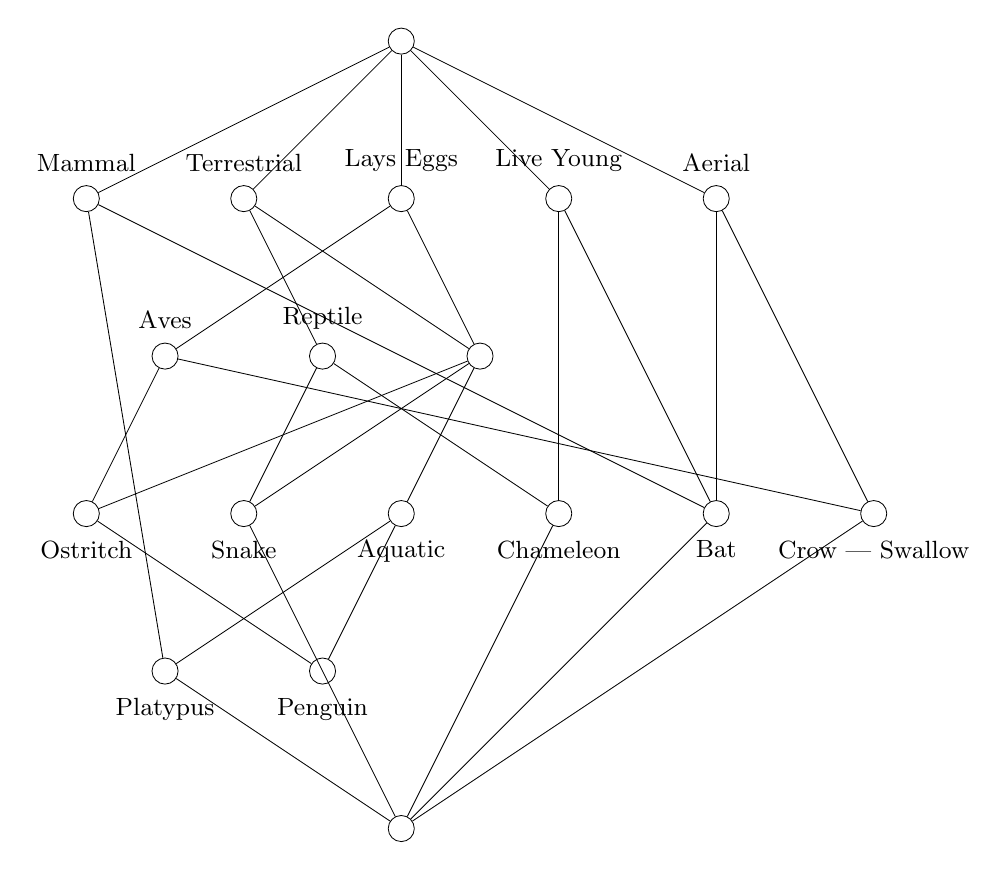
\begin{tikzpicture}[
            scale=1,
            concept/.style={circle, draw, line width=0.3pt, minimum size=0.2cm},
            label_above/.style={font=\small, above=0.05cm},
            label_below/.style={font=\small, below=0.05cm},
            line/.style={draw, line width=0.3pt}
        ]
        % Top node
        \node[concept] (root) at (0,8) {};

        % First level - characteristics
        \node[concept] (mammal) at (-4,6) {};
        \node[label_above] at (mammal.north) {Mammal};
        \node[concept] (terrestrial) at (-2,6) {};
        \node[label_above] at (terrestrial.north) {Terrestrial};
        \node[concept] (eggs) at (0,6) {};
        \node[label_above] at (eggs.north) {Lays Eggs};
        \node[concept] (young) at (2,6) {};
        \node[label_above] at (young.north) {Live Young};
        \node[concept] (aerial) at (4,6) {};
        \node[label_above] at (aerial.north) {Aerial};

        % Middle level - classifications
        \node[concept] (aves) at (-3,4) {};
        \node[label_above] at (aves.north) {Aves};

        \node[concept] (mid_empty) at (1,4) {};

        \node[concept] (reptile) at (-1,4) {};
        \node[label_above] at (reptile.north) {Reptile};

        % Lower level
        \node[concept] (ostritch) at (-4,2) {};
        \node[label_below] at (ostritch.south) {Ostritch};
        \node[concept] (snake) at (-2,2) {};
        \node[label_below] at (snake.south) {Snake};
        \node[concept] (aquatic) at (0,2) {};
        \node[label_below] at (aquatic.south) {Aquatic};
        \node[concept] (chameleon) at (2,2) {};
        \node[label_below] at (chameleon.south) {Chameleon};
        \node[concept] (bat) at (4,2) {};
        \node[label_below] at (bat.south) {Bat};
        \node[concept] (crow) at (6,2) {};
        \node[label_below] at (crow.south) {Crow | Swallow};

        % Bottom level
        \node[concept] (platypus) at (-3,0) {};
        \node[label_below] at (platypus.south) {Platypus};
        \node[concept] (penguin) at (-1,0) {};
        \node[label_below] at (penguin.south) {Penguin};

        \node[concept] (bot) at (0,-2) {};

        \draw[line] (mammal) -- (root);
        \draw[line] (terrestrial) -- (root);
        \draw[line] (eggs) -- (root);
        \draw[line] (young) -- (root);
        \draw[line] (aerial) -- (root);

        \draw[line] (eggs) -- (aves);
        \draw[line] (eggs) -- (mid_empty);
        \draw[line] (terrestrial) -- (reptile);
        \draw[line] (terrestrial) -- (mid_empty);

        \draw[line] (mammal) -- (bat);
        \draw[line] (mammal) -- (platypus);

        \draw[line] (young) -- (bat);
        \draw[line] (young) -- (chameleon);

        \draw[line] (aerial) -- (bat);
        \draw[line] (aerial) -- (crow);

        \draw[line] (aves) -- (ostritch);
        \draw[line] (aves) -- (crow);

        \draw[line] (reptile) -- (snake);
        \draw[line] (reptile) -- (chameleon);

        \draw[line] (mid_empty) -- (snake);
        \draw[line] (mid_empty) -- (ostritch);
        \draw[line] (mid_empty) -- (aquatic);

        \draw[line] (crow) -- (bot);

        \draw[line] (ostritch) -- (penguin);

        \draw[line] (aquatic) -- (penguin);
        \draw[line] (aquatic) -- (platypus);

        \draw[line] (bat) -- (bot);

        \draw[line] (snake) -- (bot);

        \draw[line] (chameleon) -- (bot);

        \draw[line] (platypus) -- (bot);

    \end{tikzpicture}
    \caption{Concept lattice for the formal context in \cref{table: formal context}.}

    \label{figure: concept lattice}
\end{figure}

\begin{table}[h]
    \centering
    \begin{tabular}{rcccccccc}
                              & \texttt{Aves} & \texttt{Mammal} & \texttt{Reptile} & \texttt{Aerial} & \texttt{Aquatic} & \texttt{Terrestrial} & \texttt{Live Young} & \texttt{Eggs} \\
        \hline
        \texttt{Bat}          &               & $\times$        &                  & $\times$        &                  &                      & $\times$            &               \\
        \texttt{Crow}         & $\times$      &                 &                  & $\times$        &                  &                      &                     & $\times$      \\
        \texttt{Ostrich}      & $\times$      &                 &                  &                 &                  & $\times$             &                     & $\times$      \\
        \texttt{Penguin}      & $\times$      &                 &                  &                 & $\times$         & $\times$             &                     & $\times$      \\
        \texttt{Platypus}     &               & $\times$        &                  &                 & $\times$         & $\times$             &                     & $\times$      \\
        \texttt{Snake}        &               &                 & $\times$         &                 &                  & $\times$             &                     & $\times$      \\
        \texttt{Swallow}      & $\times$      &                 &                  & $\times$        &                  &                      &                     & $\times$      \\
        \texttt{J. Chameleon} &               &                 & $\times$         &                 &                  & $\times$             & $\times$            &               \\
    \end{tabular}
    \vspace{10pt}
    \caption{A formal context describing animals (objects) and some of their features (attributes)}
    \label{table: formal context}
\end{table}
\clearpage

% \twocolumn

% \begin{table}
% 	\centering
% 	\begin{tabular}{r|c|c|c|c|c|c|c|c|c|c}
% 		                   & \texttt{Aves} & \texttt{Mammal} & \texttt{Reptile} & \texttt{Aerial} & \texttt{Aquatic} & \texttt{Terrestrial} & \texttt{Migratory} & \texttt{Solitary} & \texttt{Carnivore} & \texttt{Eggs} \\
% 		\hline
% 		\texttt{Bat}       &               & $\times$        &                  & $\times$        &                  &                      &                    &                   & $\times$           &               \\
% 		\texttt{Crocodile} &               &                 & $\times$         &                 & $\times$         & $\times$             &                    &                   & $\times$           & $\times$      \\
% 		\texttt{Crow}      & $\times$      &                 &                  & $\times$        &                  &                      &                    &                   &                    & $\times$      \\
% 		\texttt{Hippo}     &               & $\times$        &                  &                 & $\times$         & $\times$             &                    & $\times$          &                    &               \\
% 		\texttt{Ostrich}   & $\times$      &                 &                  &                 &                  & $\times$             &                    & $\times$          &                    & $\times$      \\
% 		\texttt{Penguin}   & $\times$      &                 &                  &                 & $\times$         & $\times$             & $\times$           &                   & $\times$           & $\times$      \\
% 		\texttt{Platypus}  &               & $\times$        &                  &                 & $\times$         & $\times$             &                    & $\times$          & $\times$           & $\times$      \\
% 		\texttt{Snake}     &               &                 & $\times$         &                 &                  & $\times$             &                    & $\times$          & $\times$           & $\times$      \\
% 		\texttt{Swallow}   & $\times$      &                 &                  & $\times$        &                  &                      & $\times$           & $\times$          & $\times$           & $\times$      \\
% 		\texttt{Whale}     &               & $\times$        &                  &                 & $\times$         &                      & $\times$           & $\times$          & $\times$           &               \\
% 	\end{tabular}
% 	\caption{Cross-table of $\K$}
% 	\label{tab:formal-context}
% \end{table}


% \begin{algorithm}
% 	\caption{Computing the tolerance partition on objects $G$}
% 	\begin{algorithmic}[1]
% 		\Require A formal context, $\FC$;
% 		\Require A set of defeasible implications, $\Delta$;
% 		\Ensure A tolerance partition $(R_0, \ldots, R_n)$ on $G$;
% 		\State $P_0 \gets G$;
% 		\State $i \gets 0$;
% 		\State $\Delta \gets \text{Material} (\Delta)$;
% 		\While {$P_{i-1} \neq P_i}$
% 			\State $P_{i+1} \gets \{g \in P_i \mid \exists \delta \in \Delta  g' \st g'\not \models \delta \}$;
% 			\State $R_i \gets P_i \setminus P_{i+1}$;
% 			\State $\Delta_i \gets \{ (\alpha \rightarrow \beta) \in \Delta \mid \exists g \in P_i \st \alpha \subseteq g'\}$;
% 			\State $\Delta \gets \Delta \setminus \Delta_i$;
% 			\EndWhile
% 			\If {$P_{i-1} = \emptyset$}
% 			\State $n \gets i-1$;
% 			\Else
% 			\State $n \gets i$;
% 			\EndIf
% 			\State \Return $\big (R_0,\ldots, R_n \big)$;
% 	\end{algorithmic}
% \end{algorithm}

% To clarify some points on
% \begin{itemize}
% 	\item Line $3$: this step turns $\Delta$ into a set of material implications;
% 	\item Line $5$: this step puts into ranking $i+1$ every object which \textbf{does not} respect $\Delta$;
% 	\item Line $7$: this sets $\Delta_i$ to be the set of formulae in $\Delta$ which have their antecedent satisfied by an object in $P_i$ (implicitly all objects in $P_i$ satisfy all formulae in $\Delta$, but we only care about the ones which have their antecedent satisfied);
% 	\item We update $\Delta$ to be those formulae which are not yet ``dealt with''.
% \end{itemize}

% \begin{algorithm}
% 	\caption{Checking entailment}
% 	\begin{algorithmic}[1]
% 		\Require A formal context, $\FC$;
% 		\Require A set of defeasible implications, $\Delta$;
% 		\Ensure A tolerance partition $(R_0, \ldots, R_n)$ on $G$;
% 		\State $P_0 \gets G$;
% 		\State $i \gets 0$;
% 		\State $\Delta \gets \text{Material} (\Delta)$;
% 		\While {$P_{i-1} \neq P_i}$
% 			\State $P_{i+1} \gets \{g \in P_i \mid \exists \delta \in \Delta  g' \st \not \Vdash \delta \}$;
% 			\State $P_i \gets P_i \setminus P_{i+1}$;
% 			\State $\Delta_i \gets \{ (\alpha \rightarrow \beta) \in \Delta \mid \exists g \in P_i \st \alpha \subseteq g'\}$;
% 			\State $\Delta \gets \Delta \setminus \Delta_i$;
% 			\EndWhile
% 			\If {$P_{i-1} = \emptyset$}
% 			\State $n \gets i-1$;
% 			\Else
% 			\State $n \gets i$;
% 			\EndIf
% 			\State \Return $\big (P_0,\ldots, P_n \big)$;
% 	\end{algorithmic}
% \end{algorithm}
% \clearpage
\small
\subsection{Risks}
\label{appendix: risks}

\begin{table}[!ht]
    \begin{tabularx}{\linewidth}{>{\justifying\arraybackslash}X>{\centering\arraybackslash}p{2cm}>{\centering\arraybackslash}p{2cm}>{\justifying\arraybackslash}X>{\justifying\arraybackslash}X>{\justifying\arraybackslash}X}
        \hline
        \textbf{Risk Description}                                                                                         & \textbf{Probability} & \textbf{Impact} & \textbf{Mitigation}                                                                                                                                                                                                & \textbf{Monitor}                                                                                            & \textbf{Manage}                                                                                                                                                                      \\
        \hline
        Not being able to achieve the research goals I set out to, (i.e. showing it cannot be done, or failing otherwise) & $0.4$                & $0.5$           & Ensure realistic goals, and that each phase of research is scrutinised to avoid realising error much later on                                                                                                      & Keep track of progress                                                                                      & In case of showing this method does not work, recognition that positive results are not necessarily required. Otherwise, consult with supervisors on how the scope may be redefined. \\
        Novel contributions of my work are published elsewhere beforehand                                                 & $0.2$                & $0.3$           & Ensure that I try publish results as soon as it is ready. Pay attention to upcoming conferences and submission dates.                                                                                              & Make sure I keep up to date with FCA publications to observe research trends.                               & Since this work is a MSc, there is no requirement for novelty. Ensure that I mention these results alongside my own.                                                                 \\
        Problem is too difficult/I get stuck on something.                                                                & $0.4$                & $0.2$           & Ensure frequent discussion with supervisors and lab-mates, asking for help when things are not clear. In addition, refer back to foundational texts to make sure my understanding of the broader field(s) is good. & A sign of not understanding things fully would be frequently making errors; monitor work for signs of this. & If I reach a point where I am not understanding the work, go back to the last point where I feel a solid grasp of the concepts, and move forward slowly.                             \\
        Suffering from fatigue, or burnout.                                                                               & $0.4$                & $0.6$           & Ensure I develop a healthy work routine, which allows me to do things outside of work, while easing fears that I'm not doing enough.                                                                               & Generally check-up on myself.                                                                               & If I do begin to feel like this, speak to supervisors about taking a short break, and then return to work later on.                                                                  \\
        Loss of work/material due to technical issues.                                                                    & $0.1$                & $0.8$           & Ensure all digital work is backed up to secure location, written work should be copied and digitised.                                                                                                              & -                                                                                                           & If this does happen, make attempts to recover lost files. Otherwise, reconstruct lost work.                                                                                          \\
        Writing/documentation challenges                                                                                  & $0.4$                & $0.3$           & Start writing early. Break thesis into manageable sections. Maintain good research notes from day one.                                                                                                             & Ensure I do regular progress checks. Keep track of references and sources properly.                         & Seek writing support if needed. Consider writing workshops or peer review groups.                                                                                                    \\
    \end{tabularx}
\end{table}

\subsection{Deliverables}
\label{appendix: deliverables}
\begin{table}[!ht]
    \begin{tabularx}{\linewidth}{>{\justifying\arraybackslash}X>{\centering\arraybackslash}p{2cm}>{\centering\arraybackslash}p{2cm}>{\justifying\arraybackslash}X}
        \hline
        \textbf{Task}                        & \textbf{Start} & \textbf{End} & \textbf{Comments}                                                               \\
        \hline
        Proposal                             & 05.10.24       & 28.10.24     & Submit draft one week before deadline                                           \\
        Background Thesis Chapters           & 01.11.24       & 31.01.25     & Submit rough outlines, and semi-incremental updates for review before deadline. \\
        Novel Results Write-Up               & 01.02.25       & 31.04.25     & While this process occurs, have meetings/feedback sessions.  results            \\
        Thesis Consolidation                 & 01.05.25       & 31.06.25     & This should be a more-or-less finished document.                                \\
        Final Review and Intention to Submit & 01.07.25       & 31.07.25     & Final adjustments and corrections                                               \\
    \end{tabularx}
\end{table}

\clearpage
\subsection{Gantt Chart}
\label{appendix: gantt chart}
\begin{table}[!ht]

    \rotatebox{270}{
        % \parbox{25cm}{
        \begin{tabular}{rlllllllllllllllllllllllllllllllllllllll}
            \textbf{2024}                  & ~     & ~     & ~     & ~     & ~     & ~     & ~     & ~     & ~     & \textbf{2025} & ~     & ~     & ~     & ~     & ~     & ~     & ~     & ~      \\
            ~                              & April & May   & June  & July  & Aug   & Sept  & Oct   & Nov   & Dec   & Jan           & Feb   & March & April & May   & June  & July  & Aug   & Sept.. \\
            ~                              & ~     & ~     & ~     & ~     & ~     & ~     & ~     & ~     & ~     &               &       &       &       &       &       &       &       &        \\
            \textbf{Literature Engagement} & \ccbM & \ccbM & \ccbM & \ccbM & \ccbM & \ccbM & \ccbM & \ccbM & \ccbM & \ccbM         & \ccbM &       &       &       &       &       &       &        \\
            \textbf{Learning}              & \ccbM & \ccbM & \ccbM & \ccbM & \ccbM &       & \ccbM & \ccbM & \ccbM & \ccbM         & \ccbM & \ccbM &       &       &       &       &       &        \\
            Learning FCA                   & ~     & \ccbS & \ccbS & ~     & \ccbS & ~     & ~     & \ccbS & ~     &               &       &       &       &       &       &       &       &        \\
            Learning KLM                   & \ccbS & ~     & \ccbS & \ccbS & \ccbS & ~     & \ccbS & ~     & ~     &               &       &       &       &       &       &       &       &        \\
            Lattice Theory + Misc          & ~     & ~     & \ccbS &       & ~     & ~     & ~     & \ccbS & \ccbS & \ccbS         &       &       &       &       &       &       &       &        \\
            \textbf{Development}           & \ccbM & \ccbM & \ccbM & \ccbM & \ccbM & \ccbM & \ccbM & \ccbM & \ccbM & \ccbM         & \ccbM & \ccbM &       &       &       &       &       &        \\
            Developing questions           & \ccbS & ~     & \ccbS & ~     & \ccbS & ~     & ~     & \ccbS & ~     &               &       & \ccbS &       &       &       &       &       &        \\
            Investigating questions        & ~     & \ccbS & ~     & \ccbS & ~     & \ccbS & \ccbS & \ccbS & \ccbS & \ccbS         & \ccbS &       &       &       &       &       &       &        \\
            \textbf{Thesis Writing}        &       &       &       &       &       &       &       &       & \ccbM & \ccbM         & \ccbM & \ccbM & \ccbM & \ccbM & \ccbM &       &       &        \\
            FCA Background                 &       &       &       &       &       &       &       &       & \ccbS &               & \ccbS &       &       &       &       &       &       &        \\
            NMR Background                 &       &       &       &       &       &       &       &       & \ccbS & \ccbS         & \ccbS &       &       &       &       &       &       &        \\
            Defeasible Implications        &       &       &       &       &       &       &       &       &       &               & \ccbS & \ccbS & \ccbS &       &       &       &       &        \\
            Rational Concepts              &       &       &       &       &       &       &       &       &       &               & \ccbS & \ccbS & \ccbS &       &       &       &       &        \\
            Consolidation                  &       &       &       &       &       &       &       &       &       &               &       &       &       & \ccbS & \ccbS & \ccbS &       &        \\
            Submit                         &       &       &       &       &       &       &       &       &       &               &       &       &       &       &       &       & \ccbS &        \\
            Proposal                       &       &       &       &       &       &       & \ccbS &       &       &               &       &       &       &       &       &       &       &        \\
            Publish second paper           &       &       &       &       &       &       &       &       &       &               &       & \ccbS & \ccbS & \ccbS & \ccbS &       &       &        \\
            \textbf{Events}                & \ccbM & \ccbM & \ccbM & \ccbM & \ccbM & \ccbM &       &       & \ccbM &               & \ccbM &       & \ccbM & \ccbM & \ccbM & \ccbM &       &        \\
            Dresden                        & \ccbS & \ccbS & \ccbS & \ccbS &       &       &       &       &       &               &       &       &       &       &       &       &       &        \\
            SACAIR                         &       &       &       &       & \ccbS & \ccbS &       &       &       &               &       &       &       &       &       &       &       &        \\
            Paper Writing                  &       &       &       &       & \ccbS & \ccbS &       &       &       &               &       &       &       &       &       &       &       &        \\
            Paper Edits                    &       &       &       &       &       &       & \ccbS &       &       &               &       &       &       &       &       &       &       &        \\
            Conference                     &       &       &       &       &       &       &       &       & \ccbS &               &       &       &       &       &       &       &       &        \\
            Cape KR                        &       &       &       &       &       &       &       &       &       &               & \ccbS &       &       &       &       &       &       &        \\
            Semester in paris              &       &       &       &       &       &       &       &       &       &               &       &       & \ccbS & \ccbS & \ccbS & \ccbS &       &
        \end{tabular}
        % \vspace{1cm}
        % \caption{\textcolor[HTML]{b6bfdb}{Blue} indicates main task, while \textcolor[HTML]{b6dbb7}{green} indicates sub-task}
        % }
    }

    \caption{\textcolor[HTML]{b6bfdb}{Blue} indicates main task, while \textcolor[HTML]{b6dbb7}{green} indicates sub-task}
\end{table}

\end{document}